\documentclass[11pt]{article}
\usepackage[margin=0.5in, landscape]{geometry}
\usepackage{tikz}
\usepackage[T1]{fontenc}
\usepackage{lmodern}

% Custom dashed underline (no ulem dependency)
\newcommand{\dashuline}[1]{%
  \tikz[baseline=(text.base)]{
    \node[inner sep=0pt, outer sep=0pt] (text) {#1};
    \draw[densely dashed, thin] (text.south west) -- (text.south east);
  }%
}
\usetikzlibrary{shapes.geometric, positioning, calc, backgrounds}

\begin{document}
\pagestyle{empty}

\begin{center}
\resizebox{\textwidth}{!}{%
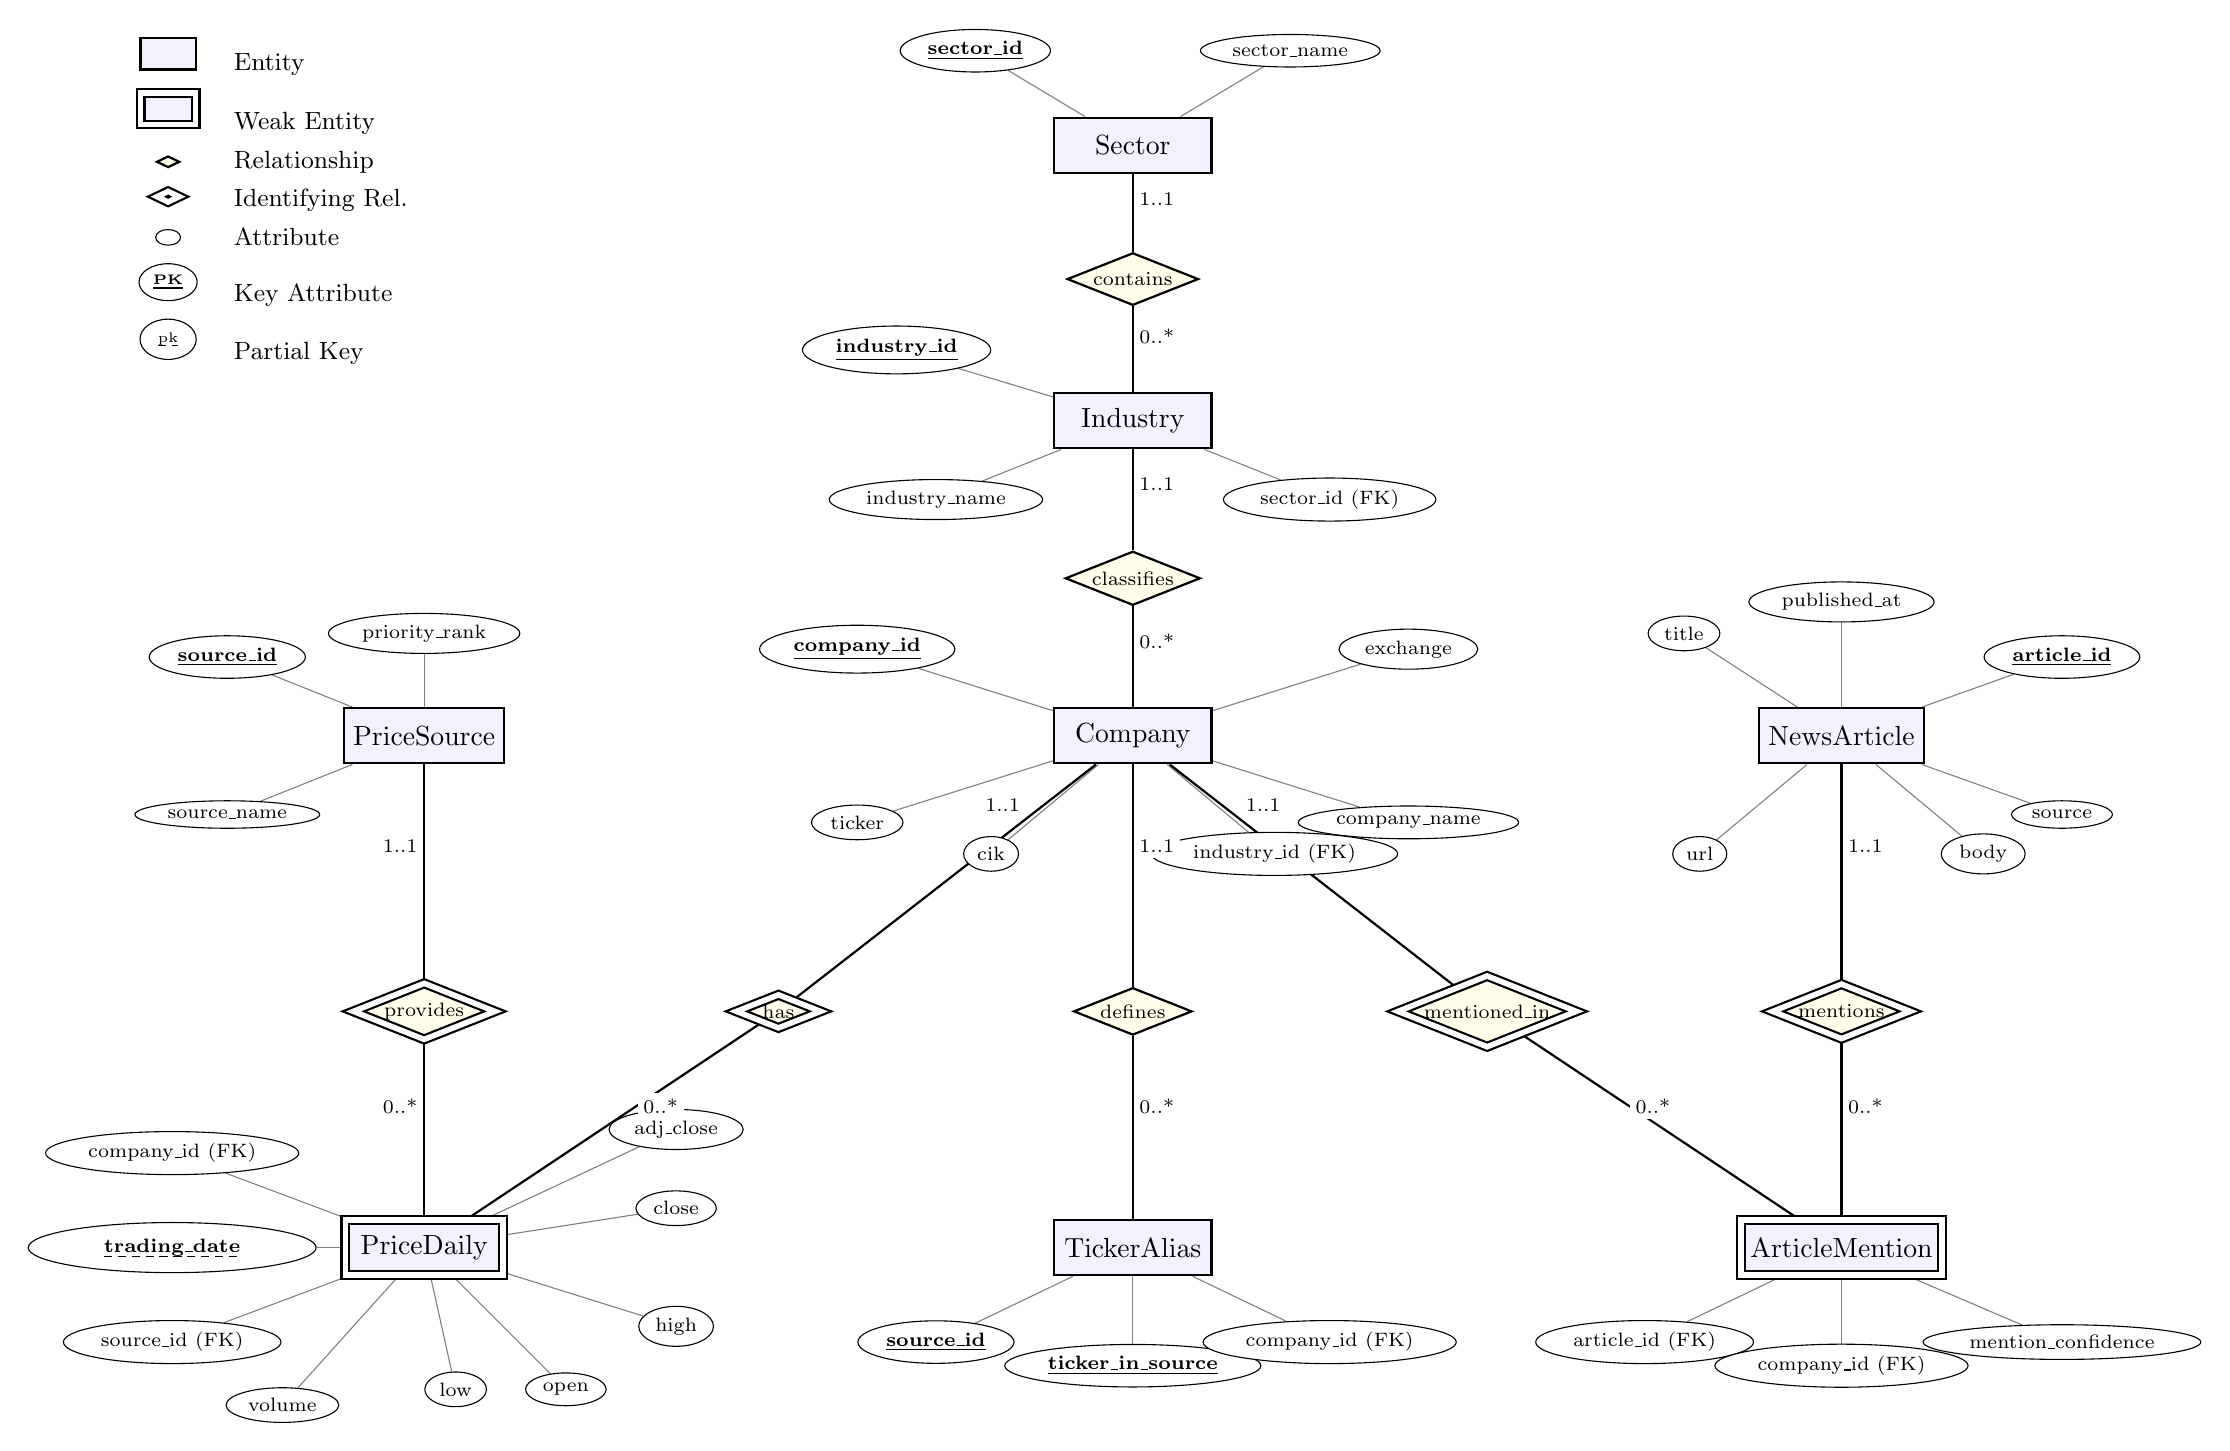
\begin{tikzpicture}[
  % --- Entity styles (from HW2) ---
  entity/.style={rectangle, draw, thick, minimum width=2cm, minimum height=0.7cm, fill=blue!5},
  weak entity/.style={rectangle, draw, thick, double, double distance=2pt,
                      minimum width=2cm, minimum height=0.7cm, fill=blue!5},
  % --- Relationship styles (from HW2) ---
  rel/.style={diamond, draw, thick, aspect=2.5, inner sep=1pt, fill=yellow!8,
              font=\footnotesize},
  ident rel/.style={diamond, draw, thick, double, double distance=2pt, aspect=2.5,
                    inner sep=1pt, fill=yellow!8, font=\footnotesize},
  % --- Attribute styles (from HW2) ---
  attr/.style={ellipse, draw, thin, inner sep=2pt, font=\scriptsize, fill=white},
  key attr/.style={attr, font=\scriptsize\bfseries},
  % --- Edge label style (from HW2) ---
  lbl/.style={font=\scriptsize, fill=white, inner sep=2pt},
  every path/.style={thick}
]

% =====================================================================
% 1) ENTITIES
% =====================================================================

% --- Sector (top center) ---
\node[entity] (sector) at (7, 12) {Sector};
\node[key attr] (s_id) at (5, 13.2) {\underline{sector\_id}};
\node[attr] (s_nm) at (9, 13.2) {sector\_name};

% --- Industry (below Sector) ---
\node[entity] (industry) at (7, 8.5) {Industry};
\node[key attr] (i_id) at (4, 9.4) {\underline{industry\_id}};
\node[attr] (i_nm) at (4.5, 7.5) {industry\_name};
\node[attr] (i_sid) at (9.5, 7.5) {sector\_id (FK)};

% --- Company (center) ---
\node[entity] (company) at (7, 4.5) {Company};
\node[key attr] (c_id) at (3.5, 5.6) {\underline{company\_id}};
\node[attr] (c_tick) at (3.5, 3.4) {ticker};
\node[attr] (c_name) at (10.5, 3.4) {company\_name};
\node[attr] (c_exch) at (10.5, 5.6) {exchange};
\node[attr] (c_cik) at (5.2, 3) {cik};
\node[attr] (c_iid) at (8.8, 3) {industry\_id (FK)};

% --- PriceSource (far left) ---
\node[entity] (pricesource) at (-2, 4.5) {PriceSource};
\node[key attr] (ps_id) at (-4.5, 5.5) {\underline{source\_id}};
\node[attr] (ps_nm) at (-4.5, 3.5) {source\_name};
\node[attr] (ps_rank) at (-2, 5.8) {priority\_rank};

% --- NewsArticle (far right) ---
\node[entity] (newsarticle) at (16, 4.5) {NewsArticle};
\node[key attr] (na_id) at (18.8, 5.5) {\underline{article\_id}};
\node[attr] (na_src) at (18.8, 3.5) {source};
\node[attr] (na_pub) at (16, 6.2) {published\_at};
\node[attr] (na_ttl) at (14, 5.8) {title};
\node[attr] (na_url) at (14.2, 3) {url};
\node[attr] (na_bod) at (17.8, 3) {body};

% --- PriceDaily (bottom left) ---
\node[weak entity] (pricedaily) at (-2, -2) {PriceDaily};
\node[attr] (pd_cid)        at (-5.2, -0.8) {company\_id (FK)};
\node[key attr] (pd_date)  at (-5.2, -2) {\dashuline{trading\_date}};
\node[attr] (pd_sid)        at (-5.2, -3.2) {source\_id (FK)};
\node[attr] (pd_o) at (-0.2, -3.8) {open};
\node[attr] (pd_h) at (1.2, -3) {high};
\node[attr] (pd_l) at (-1.6, -3.8) {low};
\node[attr] (pd_c) at (1.2, -1.5) {close};
\node[attr] (pd_ac) at (1.2, -0.5) {adj\_close};
\node[attr] (pd_v) at (-3.8, -4) {volume};

% --- TickerAlias (bottom center) ---
\node[entity] (tickeralias) at (7, -2) {TickerAlias};
\node[key attr] (ta_sid)   at (4.5, -3.2) {\underline{source\_id}};
\node[key attr] (ta_tis)  at (7, -3.5) {\underline{ticker\_in\_source}};
\node[attr] (ta_cid)       at (9.5, -3.2) {company\_id (FK)};

% --- ArticleMention (bottom right) ---
\node[weak entity] (articlemention) at (16, -2) {ArticleMention};
\node[attr] (am_aid)  at (13.5, -3.2) {article\_id (FK)};
\node[attr] (am_cid)  at (16, -3.5) {company\_id (FK)};
\node[attr] (am_mc)   at (18.8, -3.2) {mention\_confidence};

% =====================================================================
% 2) RELATIONSHIP DIAMONDS
% =====================================================================

\node[rel] (contains) at (7, 10.3) {\scriptsize contains};
\node[rel] (classifies) at (7, 6.5) {\scriptsize classifies};
\node[ident rel] (has_price) at (2.5, 1) {\scriptsize has};
\node[ident rel] (provides) at (-2, 1) {\scriptsize provides};
\node[rel] (defines) at (7, 1) {\scriptsize defines};
\node[ident rel] (mentioned) at (11.5, 1) {\scriptsize mentioned\_in};
\node[ident rel] (mentions) at (16, 1) {\scriptsize mentions};

% =====================================================================
% 3) DRAW ALL EDGES ON BACKGROUND (lines behind shapes)
% =====================================================================

\begin{pgfonlayer}{background}

  % --- Attribute edges (thin, gray, subtle) ---
  \foreach \n in {s_id, s_nm} { \draw[thin,gray] (sector) -- (\n); }
  \foreach \n in {i_id, i_nm, i_sid} { \draw[thin,gray] (industry) -- (\n); }
  \foreach \n in {c_id, c_tick, c_name, c_exch, c_cik, c_iid} { \draw[thin,gray] (company) -- (\n); }
  \foreach \n in {ps_id, ps_nm, ps_rank} { \draw[thin,gray] (pricesource) -- (\n); }
  \foreach \n in {na_id, na_src, na_pub, na_ttl, na_url, na_bod} { \draw[thin,gray] (newsarticle) -- (\n); }
  \foreach \n in {pd_cid, pd_date, pd_sid, pd_o, pd_h, pd_l, pd_c, pd_ac, pd_v} { \draw[thin,gray] (pricedaily) -- (\n); }
  \foreach \n in {ta_sid, ta_tis, ta_cid} { \draw[thin,gray] (tickeralias) -- (\n); }
  \foreach \n in {am_aid, am_cid, am_mc} { \draw[thin,gray] (articlemention) -- (\n); }

  % --- Relationship edges ---

  % Sector -- contains -- Industry
  \draw (sector) -- (contains);
  \draw (contains) -- (industry);

  % Industry -- classifies -- Company
  \draw (industry) -- (classifies);
  \draw (classifies) -- (company);

  % Company -- has -- PriceDaily
  \draw (company) -- (has_price);
  \draw (has_price) -- (pricedaily);

  % PriceSource -- provides -- PriceDaily
  \draw (pricesource) -- (provides);
  \draw (provides) -- (pricedaily);

  % Company -- defines -- TickerAlias
  \draw (company) -- (defines);
  \draw (defines) -- (tickeralias);

  % Company -- mentioned_in -- ArticleMention
  \draw (company) -- (mentioned);
  \draw (mentioned) -- (articlemention);

  % NewsArticle -- mentions -- ArticleMention
  \draw (newsarticle) -- (mentions);
  \draw (mentions) -- (articlemention);

\end{pgfonlayer}

% =====================================================================
% 4) CARDINALITY LABELS (foreground, on top of everything)
% =====================================================================

% Sector -- contains -- Industry
\node[lbl] at ($(sector)!0.4!(contains)$) [right] {1..1};
\node[lbl] at ($(contains)!0.4!(industry)$) [right] {0..*};

% Industry -- classifies -- Company
\node[lbl] at ($(industry)!0.4!(classifies)$) [right] {1..1};
\node[lbl] at ($(classifies)!0.4!(company)$) [right] {0..*};

% Company -- has -- PriceDaily
\node[lbl] at ($(company)!0.3!(has_price)$) [above left] {1..1};
\node[lbl] at ($(has_price)!0.4!(pricedaily)$) [right] {0..*};

% PriceSource -- provides -- PriceDaily
\node[lbl] at ($(pricesource)!0.4!(provides)$) [left] {1..1};
\node[lbl] at ($(provides)!0.4!(pricedaily)$) [left] {0..*};

% Company -- defines -- TickerAlias
\node[lbl] at ($(company)!0.4!(defines)$) [right] {1..1};
\node[lbl] at ($(defines)!0.4!(tickeralias)$) [right] {0..*};

% Company -- mentioned_in -- ArticleMention
\node[lbl] at ($(company)!0.3!(mentioned)$) [above right] {1..1};
\node[lbl] at ($(mentioned)!0.4!(articlemention)$) [right] {0..*};

% NewsArticle -- mentions -- ArticleMention
\node[lbl] at ($(newsarticle)!0.4!(mentions)$) [right] {1..1};
\node[lbl] at ($(mentions)!0.4!(articlemention)$) [right] {0..*};


% =====================================================================
% 5) LEGEND
% =====================================================================

\node[anchor=north west, font=\small] at (-6, 13.5) {
  \begin{tabular}{cl}
  \tikz\node[rectangle, draw, thick, fill=blue!5, minimum width=0.7cm, minimum height=0.4cm, font=\tiny] {}; & Entity \\[3pt]
  \tikz\node[rectangle, draw, thick, double, double distance=2pt, fill=blue!5, minimum width=0.7cm, minimum height=0.4cm, font=\tiny] {}; & Weak Entity \\[3pt]
  \tikz\node[diamond, draw, thick, fill=yellow!8, aspect=2, inner sep=1pt, font=\tiny] {~~}; & Relationship \\[3pt]
  \tikz\node[diamond, draw, thick, double, double distance=2pt, fill=yellow!8, aspect=2, inner sep=1pt, font=\tiny] {~~}; & Identifying Rel. \\[3pt]
  \tikz\node[ellipse, draw, thin, fill=white, inner sep=2pt, font=\tiny] {~~}; & Attribute \\[3pt]
  \tikz\node[ellipse, draw, thin, fill=white, inner sep=2pt, font=\tiny\bfseries] {\underline{PK}}; & Key Attribute \\[3pt]
  \tikz\node[ellipse, draw, thin, fill=white, inner sep=2pt, font=\tiny] {\dashuline{pk}}; & Partial Key \\
  \end{tabular}
};

\end{tikzpicture}%
}% end resizebox
\end{center}

\end{document}